%
% Revisão da Literatura
%

\chapter{Revisão da Literatura}

% 
% Aprendizado de máquina
%

%%%%%%
% TODO verificar os TODO e os FIXME antes da próxima" "release"
%%%%%%

\newcommand{\vect}[1]{\mathbf{#1}}
\newcommand{\norma}[1]{\lVert #1 \rVert}

% Usar Inductive Principles for Learning from Data como referência "dos
% tópicos" para esse assunto, e também o "Uma Introdução às Support Vector
% Machines".
% Tomar cuidado em manter a consistência entre as diferentes notações
% usadas entre as referências.
%
% - A teoria do aprendizado estatístico
% - Métodos paramétricos
% - Métodos adaptativos
% - Risco esperado, risco estatístico
% - Classificação binária
% - Classificação multi-classes
% - Como adaptar um classificador binário para um problema multi-classes
%   (Pairwise, e esqueciooutro)
%
% Apresentar (brevemente) algumas outras técnicas também:
% (lista baseada em wiki/Supervised_learning#Approaches_and_algorithms)
% - redes neurais artificiais
% - inferência bayesiana
% - ...
%
% FIXME Aqui realmente estou em dúvida. Devemos apresentar TODAS as
% técnicas, uma por parágrafo, ou apresentar uma a uma?
% -- Pelo que tenho visto em outras monografias, não é necessário
%  apresentar o estado da arte da área de aprendizado (Ver Trabalhos
%  Relacionados no Google Docs)

Um dos comportamentos mais característicos de sistemas computacionais que possam ser considerados inteligentes é o de melhorar o seu desempenho para resolver algum problema quando este se depara com a mesma situação por mais de uma vez ~\cite{luger2004inteligencia}. ~\apudonline{simon1983should}{luger2004inteligencia} define o conceito de aprendizado de máquina como sendo qualquer mudança que melhore o seu desempenho na segunda vez que ele repetir a mesma tarefa, ou em uma tarefa da mesma população.

Nem sempre é possível obter um resultado ótimo para novas situações, pois na maioria dos casos não é possível apresentar a um sistema a quantidade de exemplos (ou experiências anteriores) necessárias para representar todos os casos possíveis. Por isso, as técnicas de aprendizado fazem uso da inferência indutiva, que consiste em prever novas situações baseando-se em um conjunto particular de exemplos~\cite{luger2004inteligencia}.

A construção da hipótese no aprendizado indutivo ocorre por meio da exposição de exemplos ao algoritmo de indução, sendo este processo chamado de treinamento. O processo de atribuir rótulos ou classes a novos exemplos é chamado de classificação. Porém, se o conjunto de exemplos usado para a indução for muito pequeno ou pouco representativo, há o risco de que as hipóteses escolhidas não descrevam corretamente novas situações e o sistema inteligente traga resultados incorretos~\cite[p. 90]{rezende2003sistemas}.

Sistemas de aprendizado de máquina podem ser divididos em dois tipos, dependendo de como são realizadas suas respectivas etapas de treinamento: supervisionados e não-supervisionados.

O aprendizado supervisionado é aquele em que há exemplos pré-existentes e estes já possuem rótulos. Tais rótulos podem ter sido atribuídos por um especialista no domínio ou representam resultados de experiências anteriores do sistema. Um classificador baseado em aprendizado supervisionado deve tentar estabelecer uma hipótese que seja genérica a ponto de que o algoritmo possa classificar corretamente novos casos. Uma hipótese muito genérica pode resultar em uma classificação inadequada (\emph{underfitting} --- sub-ajuste), ao passo que uma hipótese que descreva corretamente apenas os exemplos que foram usados para o treinamento pode ter um desempenho inadequado em casos novos (\emph{overfitting} --- sobre-ajuste).

No aprendizado não-supervisionado, não há rótulos para atribuir aos exemplos, pois o objetivo do algoritmo é encontrar grupos de exemplos que possuam semelhança entre eles. As técnicas deste modelo são referenciadas como sendo ``técnicas de agrupamento'' ou \emph{clustering}~\cite{rezende2003sistemas}.
%FIXME terminar não-supervisionado (dar uma olhada no livro do Luger)

\subsection{Técnicas de aprendizado supervisionado}

Dentre as técnicas de aprendizado supervisionado mais populares estão, não exclusivamente supervisionados, Redes Neurais Artificiais, Máquinas de Vetores de Suporte (SVMs --- \emph{Support Vector Machines}), $k$ Vizinhos Mais Próximos ($k$-NN --- \emph{k-Nearest Neighbors}) e \emph{Naïve Bayes}.

% FIXME faltou descrever GGM, RBF, Redes Bayesianas e árvores de decisão

$k$-NN é uma técnica de aprendizado supervisionado que utiliza todos os exemplos durante a etapa de classificação, tendo assim pouco custo para treinamento e alto custo para classificação. Para classificar as entradas, comumente mede-se a distância euclideana de todos os exemplos da base e então é selecionada a classe que predomina no grupo de $N$ elementos que estiver mais próximo\cite{tan2006effective}.

Há também as técnicas baseadas em Árvores de Decisão, que visam a indução de uma árvore que represente o conhecimento. Os ramos desta árvore indicam conjunções (tanto de testes binários quanto multivalorados), ao passo que as folhas representam classficações. Para classificar novos casos simplemente percorre-se a árvore de decisão avaliando cada conjunção em cada ramo e seguindo para a subárvore adequada, quando atinge-se as folhas é encontrada a classe final~\cite{de-categorizacao}. Esta técnica possui a vantagem de que sua forma de representação permita que humanos compreendam com facilidade o conteúdo que ela representa~\cite[p. 52]{mitchell1997machine}. Os algoritmos para indução de árvores de decisão mais populares são ID3~\cite{quinlan1986induction}, C4.5~\cite{quinlan1993programs} e CART~\cite{breiman1984classification}.

\emph{Naïve Bayes} é um algoritmo de aprendizado supervisionado, que
utiliza probabilidade para a classificação, supondo que as variáveis de cada
exemplo são condicionalmente independentes \cite{de-categorizacao}, as
probabilidades são calculadas de acordo com o Teorema de Bayes
\cite{kim2003poisson}, para a classificação de um elemento desconhecido, é
calculada a probabilidade de todas as classes e a classe com maior
probabilidade é escolhida como rótulo para o elemento desconhecido.
~\cite{pardo2002aprendizado}

A técnica de Redes Neurais Artificiais (RNAs) baseou-se originalmente no comportamento de neurônios observados na natureza. Uma RNA é formada por uma rede com grande quantidade de unidades de aprendizado, que recebem uma série de valores contínuos que fazem parte dos exemplos de treinamento, produzindo então um valor contínuo, que por sua vez pode ser repassado para outros agrupamentos dessas unidades ou ser utilizado para reajustar pesos internos, permitindo que novos exemplos sejam classificados em iterações futuras.~\cite[p. 81-86]{mitchell1997machine}

SVMs é uma técnica modelada como um problema de otimização que tenta encontrar, no espaço do conjunto de exemplos, um hiperplano que separe com maior margem os exemplos de cada uma das duas classes. Em razão da aplicação desta técnica em parte da metodologia proposta neste trabalho, será feita uma apresentação mais detalhada a partir da seção \ref{sec:svm}). Antes disso, as seções a seguir buscam apresentar os conceitos e terminologia comumente utilizados na apresentação das SVMs.

\subsection{Formalização do aprendizado supervisionado}

Como já brevemente apresentado, no problema de aprendizado supervisionado existe a figura de um professor que indica qual é o rótulo correto para cada exemplo. Cada exemplo pode ser descrito na forma $(\vect{x}_i, y_i)$, aonde $\vect{x}_i$ denota um exemplo e $y_i$ seria a classe ou rótulo. Após o processo de treinamento, pode-se descrever o classificador como uma função $f(\vect{x}) = y$, sendo que $\vect{x}$ não é necessariamente um dos valores de $\vect{x}_i$ \apud{haykin1994neural}{lorena2003introducaoas}.

Os valores dos rótulos que os exemplos podem assumir podem ser discretos ou contínuos. Para o caso dos contínuos assume-se que é possível obter $1,\dotsc,k$ valores. Quando $k = 2$, o problema é denominado como sendo de ``classificação binária''. Quando $k > 2$ denomina-se como sendo um problemas de ``classificação multiclasses''.

As amostras $\vect{x}_i$, são representadas por vetores com as características (também denominadas atributos) de cada exemplo. Cada amostra $\vect{x}_i$ possui $m$ atributos e também pode ser representada como $\vect{x}_i = (x_{i1},\dotsc,x_{im})$. Os atributos podem assumir dois tipos de valores: nominais ou contínuos. Os atributos nominais assumem valores que não possuem ordem entre si e sua representação tem função simbólica (por exemplo: segunda-feira, azul, não). Os atributos contínuos possuem ordem entre si e comumente representam valores dos domínios $\mathbb{Z}$ e $\mathbb{R}$.

O objetivo de uma técnica de aprendizado de máquina é obter uma função $f(\vect{x}) = y$ que obtenha um $y$ adequado aos exemplos que foram apresentados pelo professor por meio de indução~\cite{osuna1997support}.

% parece ser muito pouco conteúdo, porém mais detalhes como (overfitting) ou
% (como avaliar o desempenho de alguma técnica de AM) já foram (acima) ou serão
% (em classificação de textos).

\subsection{\emph{Support Vector Machines} --- SVMs}\label{sec:svm}
%
%   - problema primal
%   - problema dual (e teoria "dos lagrangianos")
%   - vetores de suporte
%   - SVM com margens rígidas
%   - SVM com margens flexíveis (E_i)
%   - kernels (RBF gaussiano etc)

A técnica de aprendizado de máquina supervisionado conhecida como \emph{Support Vector Machines} (SVM), ou Máquinas de Vetores de Suporte, foi introduzida por Boser, Guyon e Vapnik em 1992 com a publica\c{c}ão de \emph{A training algorithm for optimal margin classifiers}\nocite{boser1992training}, que baseia-se no trabalho da teoria do aprendizado estatístico desenvolvida por Vapnik \emph{et al}. desde a década de 1960~\cite{antos2003data}.

SVMs partem do princípio de que quanto mais largas as margens de um hiperplano separador de uma fun\c{c}ão, (explicado na se\c{c}ão \ref{sec:aprendizado} por meio do conceito de minimiza\c{c}ão do risco estrutural), maiores são as chances de que ele possa prover uma boa generaliza\c{c}ão dos dados que estão sendo usados como exemplo \cite{chapelle2002choosing}. Desta forma, SVMs buscam encontrar um hiperplano descrito por $f(\vect{x}) = \vect{w}\cdot\vect{x} + b = 0$ que tenha maior margem entre as classes e menor complexidade estrutural por meio da resolu\c{c}ão de um problema de otimiza\c{c}ão.

Para encontrar o hiperplano separador ideal, é necessário utilizar, pelo menos, dois pontos do conjunto de exemplos. Sejam $\vect{x}_1$ e $\vect{x}_2$ dois exemplos do conjunto de treinamento $T$ que possui um conjunto de exemplos $X$ com rótulos do conjunto de exemplos $Y = \{-1, +1\}$, sendo que cada um deles fica em um lado diferente do hiperplano separador. Para encontrar o hiperplano separador $f(\vect{x}) = \vect{w}\cdot\vect{x} + b = 0$ entre $\vect{x}_1$ e $\vect{x}_2$, é necessário conhecer o vetor $\vect{w}$, que deve ser normal a este hiperplano e que é usado para calcular o tamanho da margem.

\begin{figure}[htp!]
  \centering
  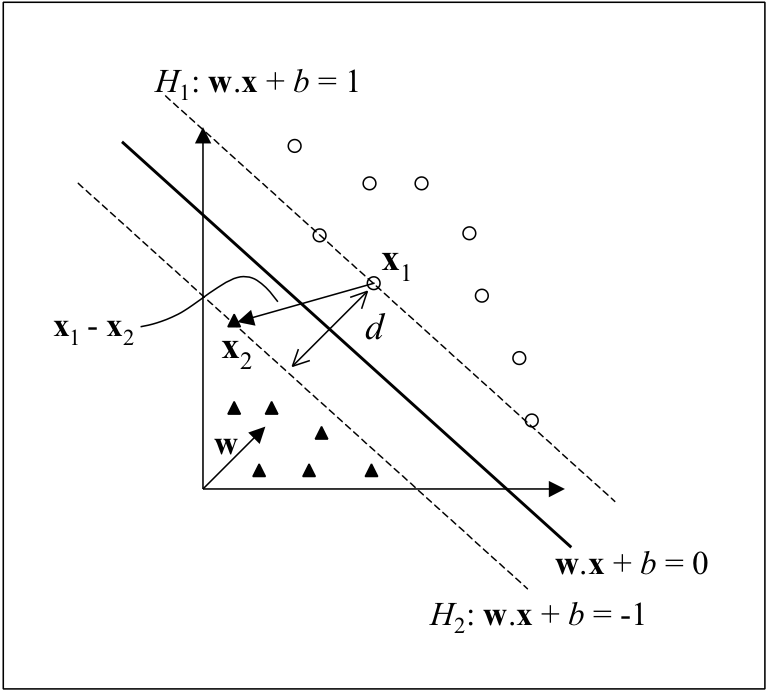
\includegraphics[width=0.5\textwidth]{img/fig-hiperplanos.png}
  \figinfox{Hiperplano separador e margens}{LORENA, 2003}
  \label{fig:hiperplanos}
\end{figure}

Como um dos objetivos do problema de otimização é obter uma margem larga entre os exemplos, pode-se restringir a busca por $\vect{w}$ apenas em termos do cálculo do tamanho da margem. Para isso, é necessário calcular a distância entre dois hiperplanos que são formados pelos exemplos $\vect{x}_1$ e $\vect{x}_2$. Sejam $H_1: \vect{w}\cdot\vect{x} + b = +1$ e $H2: \vect{w}\cdot\vect{x} +b = -1$ dois hiperplanos que ficam paralelamente acima e abaixo, respectivamente, do hiperplano separador. Além disso, assume-se que $H_1$ passa por $\vect{x}_1$ e $H_2$ passa por $\vect{x}_2$. A figura \ref{fig:hiperplanos} mostra a relação entre os hiperplanos e os pontos $\vect{x}_1$ e $\vect{x}_2$.

Conhecendo os hiperplanos, agora é possível calcular a distância entre os hiperplanos que servem de fronteira entre cada ponta da margem do hiperplano separador. A equação \ref{eq:projecao_w} apresenta o cálculo necessário para projetar $\vect{x}_1 - \vect{x}_2$ na direção de $\vect{w}$, que é perpendicular ao hiperplano separador $\vect{w}\cdot\vect{x} + b = 0$.
\begin{equation}\label{eq:projecao_w}
  (x_1 - x_2)
    \left(
      \frac{ \vect{w} }{ \norma{\vect{w}} }
      \cdot
      \frac{(x_1 - x_2)}{ \norma{\vect{x}_1 - \vect{x}_2} }
    \right)
\end{equation}

Sabendo que $\vect{w}\cdot\vect{x}_1 + b = +1$ e $\vect{w}\cdot\vect{x}_2 + b = -1$, e levando em conta que deseja-se saber o comprimento do vetor resultante, é usada a norma da equação \ref{eq:projecao_w} para chegar à equação \ref{eq:projecao_w2}, que indica a distância $d$ utilizada na figura \ref{fig:hiperplanos}:
\begin{equation}\label{eq:projecao_w2}
  d = \frac{2}{\norma{\vect{w}}}
\end{equation}

Portanto, as distâncias entre $\vect{x}_1$, $\vect{x}_2$ e o hiperplano separador $\vect{w}\cdot\vect{x} + b = 0$ são $\frac{1}{\norma{\vect{w}}}$, e com isso, é possível definir o problema de otimização como definido pelo problema de otimização da equação \ref{eq:max_w0}. A restrição \ref{eq:max_w1} indica que $H_1$ e $H_2$ devem passar, respectivamente, pelos vetores $\vect{x}_1$ e $\vect{x}_2$.
\begin{eqnarray}
& \label{eq:max_w0}\operatorname{Maximizar} & \frac{2}{\norma{\vect{w}}} \\
& \label{eq:max_w1} \operatorname{sujeito\;a} & y_i(\vect{w}\cdot\vect{x}_i + b) - 1 \ge 0 \quad i = 1,\dotsc,n.
\end{eqnarray}

No problema de maximização da equação \ref{eq:max_w0}, $\frac{2}{\norma{\vect{w}}}$ pode ser descrito como um problema de minimização de $\norma{\vect{w}}^2/{2}$:
\begin{eqnarray}
& \label{eq:min_w0}\operatorname{Minimizar} & \frac{\norma{\vect{w}}^2}{2} \\
& \nonumber \operatorname{sujeito\;a} & y_i(\vect{w}\cdot\vect{x}_i + b) - 1 \ge 0 \quad i = 1,\dotsc,n.
\end{eqnarray}

%% FIXME rev Neusa: Que função é essa? [função de lagrange] Pelo menos deve colocar uma referência

A partir deste ponto, o problema da equação \ref{eq:min_w0} pode ser resolvido com técnicas de programação quadrática (PQ) \cite{osuna1997support}. Este tipo de problema pode ser solucionado utilizando uma função Lagrangiana e adicionando as restrições à função objetivo junto com os multiplicadores de Lagrange $\alpha_i$ \cite{smola2000advances} (a técnica conhecida como “multiplicadores de Lagrange” tem como objetivo simplificar a busca pelo ponto ótimo de um problema de otimização unindo a função objetivo às funções de restrição). A equação \ref{eq:lagrange0} deve ser minimizada, o que significa maximizar $\alpha_i$ e minimizar $\vect{w}$ e $b$. O problema é representado desta forma para que a restrição (da equação \ref{eq:max_w1}) possa ser representada na forma dos multiplicadores $\alpha_i$, o que facilita os cálculos mais adiante, e também porque os dados de treinamento apenas aparecem na forma de produtos entre vetores \cite{burges1998tutorial}, o que permite o uso de \emph{kernels} (seção \ref{sec:naolinear}).
\begin{equation}\label{eq:lagrange0}
  L(\vect{w}, b, \vect{\alpha}) = \frac{1}{2}\norma{\vect{w}}^2 - 
       \sum_{i=1}^n{\alpha_i(y_i(\vect{w}\cdot\vect{x}_i + b) - 1)}
\end{equation}

Tem-se ponto de sela, então:
\begin{eqnarray}\label{eq:sela}
  \frac{\partial{L}}{\partial{b}} = 0 & \text{e} & \frac{\partial{L}}{\partial{\vect{w}}} = 0
\end{eqnarray}
E com isso:
\begin{eqnarray}
&  \label{eq:lagsum0}  \sum_{i=1}^n{\alpha_i y_i} = 0 \\
&  \label{eq:lagsum1}  \vect{w} = \sum_{i=1}^n{\alpha_i y_i\vect{x}_i}
\end{eqnarray}

Assim, substituindo equações \ref{eq:lagsum0} e \ref{eq:lagsum1}, é possível formular o problema de otimização:
\begin{eqnarray}\label{eq:maxalpha}
\begin{array}{rl}
   %\operatorname*{Maximizar}_{\alpha}
   \underset{\alpha}{\operatorname{Maximizar}}
   & \sum_{i=1}^n{\alpha_i - \frac{1}{2}}
                            \sum_{i,j=1}^n{\alpha_i\alpha_j y_i y_j(\vect{x}_i\cdot\vect{x}_j)} \\
\operatorname{sujeito\;a} &
  \begin{cases}
    \alpha_i \geqslant 0, \forall{i} = 1,\dotsc,n \\
    \sum_{i=1}^n{\alpha_i y_i} = 0
  \end{cases}
\end{array}
\end{eqnarray}

A equação \ref{eq:maxalpha} é denominada a forma dual do problema, ao passo que a formulação original (equação \ref{eq:min_w0}), é denominada a forma primal, baseada no trabalho de \apudonline{fletcher1987practical}{burges1998tutorial}. Chama-se de forma dual a disposição do problema de otimização que envolve os mesmos coeficientes, mas são dispostos de maneira diferente do problema original (chamada de primal), formando um problema que tem ponto ótimo próximo ao da formulação original~\cite{puccini1990introducao}.

% TODO REV Marcio pg16, "quais são as condições [de KKT]"

É possível utilizar as condições Karush-Kuhn-Tucker (KKT), que indicam em quais situações um problema de otimização pode garantidamente chegar a um ponto ótimo, descritas em \citeonline[proposição 3.3.1]{bertsekas-nonlinear}, visto que o problema de otimização \ref{eq:maxalpha} possui restrições lineares e a função objetivo é convexa \cite{burges1998tutorial}. Assim, segundo essas condições, é possível encontrar $\vect{w^*}$ e $b^*$ que podem ser considerados solução ótima para o problema a partir da solução do problema dual ao encontrar $\alpha_i^*$:
\begin{equation}\label{eq:dualalpha}
  \alpha_i^*(y_i(\vect{w^*}\cdot\vect{x}_i+b^*) - 1) = 0, \forall{i}=1,\dotsc,n
\end{equation}

Na equação \ref{eq:dualalpha}, $\alpha_i^*$ é diferente de zero apenas para os valores que tocam a borda das margens do hiperplano de decisão ($H_1$ e $H_2$). Assim, esses dados são chamados de ``vetores de suporte'', pois são os dados mais significativos para a localização de hiperplano $\vect{w}\cdot\vect{x} + b = 0$.

E para calcular $b^*$, de acordo com com a equação \ref{eq:dualalpha}:
\begin{equation}
  b^* = \frac{1}{n_{SV}}\sum_{x_j \in SV}{\frac{1}{y_j} - \vect{w^*}\cdot\vect{x}_j}
\end{equation} Onde $n_{SV}$ é o número de vetores de suporte e $SV$ o conjunto dos mesmos.

% ALELUIA!!!!!!!!!!!! PQPQPQPQPQPQPQP!!!
Finalmente, obtém-se a seguinte função classificadora:
\begin{equation}\label{eq:classificadora}
  g(\vect{x}) = \operatorname{sinal}(f(\vect{x}))
              = \operatorname{sinal}\left(
                  \sum_{x_i \in SV}{y_i\alpha_i^*\vect{x}_i\cdot\vect{x}+b^*}
                \right)
\end{equation}

\subsubsection{Margens suaves}

% seção está incompleta, não explica bem como o erro é tratado em si

Para tratar os casos em que há \emph{outliers} nos exemplos, ou seja, dados que estão rotulados incorretamente ou com algum ruído, utiliza-se a técnica de margens suaves, que é uma saída mais simples que SVMs não-lineares \cite{burges1998tutorial}.

%% TODO FIXME rev Neusa, no trecho "mais simples que SVMs não-lineares": "qual é a complexidade de SVMs não lineares"?

Utiliza-se variáveis de folga $\xi_i$ para cada exemplo $\vect{x}_i$ do conjunto de treinamento. Essas variáveis são adicionadas à restrição do problema primal:
\begin{equation}\label{eq:restrsuave}
  y_i(\vect{w}\cdot\vect{x}_i+b) \geqslant 1 - \xi_i,\quad\forall{i}=1,\dotsc,n
\end{equation}

Ao passo que a função objetivo é reformulada como:
\begin{equation}
  \underset{\vect{w}, b, \vect{\xi}}{\operatorname{Minimizar}}\quad
         \frac{1}{2}\norma{\vect{w}}^2+C\left(\sum_{i=1}^n{\xi_i}\right)
\end{equation}

A constante $C$ impõe uma penalização à violação das restrições descritas na equação \ref{eq:restrsuave} do problema de otimização. O valor desta constante é definida pelo usuário e sua definição depende de testes baseados no conjunto de treinamento. Algumas abordagens para a escolha deste parâmetro foram apresentadas por \citeonline{chapelle2002choosing}, \citeonline{cherkassky2004practical}, \citeonline{quang2002evolving} e \citeonline{ben2010user}.

% FIXME descrever o método de busca em grade de ben2010user, pois é o que
% usamos

\subsubsection{Classificação não-linear}\label{sec:naolinear}

Segundo o teorema de \citeonline{cover1965geometrical}, as chances de que um conjunto de exemplos não linearmente separável possa ser separado por um hiperplano é grande quando este é disposto em um espaço de maior dimensionalidade. Assim, a implementação de SVMs utiliza esta técnica para conseguir separar dados ainda de maneira linear~\cite{burges1998tutorial}.

Com isso, os dois vetores $\vect{x}$ e $\vect{x}_i$, que são utilizados na função de decisão (equação \ref{eq:classificadora}), são convertidos para o espaço de maior dimensão por um mapeamento $\vect{\Phi}: X \rightarrow \Im$, aonde $X$ é o espaço de entrada e $\Im$ o espaço de características.

Adicionalmente, o produto entre os vetores $\vect{x}$ e $\vect{x}_i$ é representado como uma função $K(\vect{x}_i, \vect{x}_j) = \vect{\Phi}(\vect{x}_i)\cdot\vect{\Phi}(\vect{x}_j)$. Esta função é chamada de \emph{função kernel} e tem por finalidade permitir o uso de funções que atentem às condições definidas pelo teorema de Mercer \cite[p. 141]{burges1998tutorial}. Esta forma de representação permite que se use estas funções de kernel dentro da implementação de uma SVM sem a necessidade de conhecimento dos detalhes internos das mesmas. O quadro \ref{quadro:kernels} apresenta alguns dos kernels mais populares utilizados com SVMs~\cite{lorena2003introducaoas}.

\begin{table}[htp]
\centering
\hspace{-2cm} % FIXME arrumar no template
\quadro{Funções de kernel comumente usadas}\label{quadro:kernels}
\begin{tabular}{|c|c|c|}
\hline
Tipo de kernel & Função & Parâmetros \\
\hline
Polinomial & $(\delta(\vect{x}_i\cdot\vect{x}_j)+\kappa)^d$ & $\delta$, $\kappa$, e $d$ \\
Gaussiano (ou RBF) & $\exp(-\sigma\norma{\vect{x}_i-\vect{x}_j}^2)$ & $\sigma$ \\
Sigmoidal & $\tanh(\delta(\vect{x}_i\cdot\vect{x}_j)+\kappa)$ & $\delta$ e $\kappa$ \\
\hline
\end{tabular} \end{table}

\subsubsection{Classificação multiclasses}\label{sec:svmmulti}

% hsu2002comparison

Como SVMs fazem classificação binária, é necessário o uso de alguma técnica para adaptar problemas de classificação multiclasses. As mais populares são um contra todos (\emph{one-against-all}) e um contra um (\emph{one-against-one}).

Na técnica um contra todos, uma SVM é treinada para cada classe contra todas as outras classes ao mesmo tempo. \citeonline{vapnik1998statistical} propôs uma extensão a esta técnica para utilizar os valores contínuos de cada SVM (ao invés do retornado por $\operatorname{sinal}$) e ordenar as classes descendentemente de acordo com o módulo da classificação de cada uma~\cite{abe2003analysis}.

Na técnica de classificação um contra um, também chamada de \emph{pairwise}, cada classe é treinada contra outra classe do problema, sendo a classe selecionada a que foi selecionada mais vezes nas classificações contra todas as outras classes. Isso resulta, em um problema de classificação de $n$ classes, em $n(n - 1)/2$ SVMs \cite{kressel1999pairwise}.

% TODO há mais técnicas interessantes (as baseadas em árvore de decisão e
% all-together), talvez apontar desempenho delas etc etc

%%\subsubsubsection{Complexidade computacional}
%% tratar

%%\subsubsubsection{Implementações}
% abandonada por falta de tempo, vamos citar apenas a libsvm na metodologia
% libsvm 
% PyML
% svm-light
% svm-perf



\section{Virtualização}

% introdução
% terminologia (host, guest, hypervisor, cloud)
% ferramentas
% utilizar descrição de: http://libvirt.org/goals.html
% 

\subsection{\emph{libVirt}}\label{sec:libvirt}

% uma descrição mais detalhada, 

A \emph{libVirt} é um conjunto de ferramentas que visa prover uma abstração
uniforme para gerenciamento de máquinas virtuais de maneira independente da
da aplicação de virtualização que está sendo utilizada. Seu desenvolvimento
foi iniciado em 2005 pela empresa Red Hat e inicialmente chamava-se
\emph{libxen} (indicando assim que era uma abstração específica para a
ferramenta \emph{Xen}), porém teve seu nome alterado para \emph{libVirt} em
2006, de maneira a refletir o interesse em suportar mais ferramentas de
virtualização \apud{gitlibvirt}{eriksson2009virtualization}.

\subsection{Interface de programação}


